\documentclass[11pt,preprint]{elsarticle}

\usepackage{lmodern}
%%%% My spacing
\usepackage{setspace}
\setstretch{1.2}
\DeclareMathSizes{12}{14}{10}{10}

% Wrap around which gives all figures included the [H] command, or places it "here". This can be tedious to code in Rmarkdown.
\usepackage{float}
\let\origfigure\figure
\let\endorigfigure\endfigure
\renewenvironment{figure}[1][2] {
    \expandafter\origfigure\expandafter[H]
} {
    \endorigfigure
}

\let\origtable\table
\let\endorigtable\endtable
\renewenvironment{table}[1][2] {
    \expandafter\origtable\expandafter[H]
} {
    \endorigtable
}


\usepackage{ifxetex,ifluatex}
\usepackage{fixltx2e} % provides \textsubscript
\ifnum 0\ifxetex 1\fi\ifluatex 1\fi=0 % if pdftex
  \usepackage[T1]{fontenc}
  \usepackage[utf8]{inputenc}
\else % if luatex or xelatex
  \ifxetex
    \usepackage{mathspec}
    \usepackage{xltxtra,xunicode}
  \else
    \usepackage{fontspec}
  \fi
  \defaultfontfeatures{Mapping=tex-text,Scale=MatchLowercase}
  \newcommand{\euro}{€}
\fi

\usepackage{amssymb, amsmath, amsthm, amsfonts}

\def\bibsection{\section*{References}} %%% Make "References" appear before bibliography


\usepackage[numbers]{natbib}

\usepackage{longtable}
\usepackage[margin=2.3cm,bottom=2cm,top=2.5cm, includefoot]{geometry}
\usepackage{fancyhdr}
\usepackage[bottom, hang, flushmargin]{footmisc}
\usepackage{graphicx}
\numberwithin{equation}{section}
\numberwithin{figure}{section}
\numberwithin{table}{section}
\setlength{\parindent}{0cm}
\setlength{\parskip}{1.3ex plus 0.5ex minus 0.3ex}
\usepackage{textcomp}
\renewcommand{\headrulewidth}{0.2pt}
\renewcommand{\footrulewidth}{0.3pt}

\usepackage{array}
\newcolumntype{x}[1]{>{\centering\arraybackslash\hspace{0pt}}p{#1}}

%%%%  Remove the "preprint submitted to" part. Don't worry about this either, it just looks better without it:
\makeatletter
\def\ps@pprintTitle{%
  \let\@oddhead\@empty
  \let\@evenhead\@empty
  \let\@oddfoot\@empty
  \let\@evenfoot\@oddfoot
}
\makeatother

 \def\tightlist{} % This allows for subbullets!

\usepackage{hyperref}
\hypersetup{breaklinks=true,
            bookmarks=true,
            colorlinks=true,
            citecolor=blue,
            urlcolor=blue,
            linkcolor=blue,
            pdfborder={0 0 0}}


% The following packages allow huxtable to work:
\usepackage{siunitx}
\usepackage{multirow}
\usepackage{hhline}
\usepackage{calc}
\usepackage{tabularx}
\usepackage{booktabs}
\usepackage{caption}


\newenvironment{columns}[1][]{}{}

\newenvironment{column}[1]{\begin{minipage}{#1}\ignorespaces}{%
\end{minipage}
\ifhmode\unskip\fi
\aftergroup\useignorespacesandallpars}

\def\useignorespacesandallpars#1\ignorespaces\fi{%
#1\fi\ignorespacesandallpars}

\makeatletter
\def\ignorespacesandallpars{%
  \@ifnextchar\par
    {\expandafter\ignorespacesandallpars\@gobble}%
    {}%
}
\makeatother


% definitions for citeproc citations
\NewDocumentCommand\citeproctext{}{}
\NewDocumentCommand\citeproc{mm}{%
\href{\#cite.\detokenize{#1}}{#2}\nocite{#1}}

\makeatletter
% allow citations to break across lines
\let\@cite@ofmt\@firstofone
% avoid brackets around text for \cite:
\def\@biblabel#1{}
\def\@cite#1#2{{#1\if@tempswa , #2\fi}}
\makeatother
\newlength{\cslhangindent}
\setlength{\cslhangindent}{1.5em}
\newlength{\csllabelwidth}
\setlength{\csllabelwidth}{3em}
\newenvironment{CSLReferences}[2] % #1 hanging-indent, #2 entry-spacing
{\begin{list}{}{%
	\setlength{\itemindent}{0pt}
	\setlength{\leftmargin}{0pt}
	\setlength{\parsep}{0pt}
	% turn on hanging indent if param 1 is 1
	\ifodd #1
	\setlength{\leftmargin}{\cslhangindent}
	\setlength{\itemindent}{-1\cslhangindent}
	\fi
	% set entry spacing
	\setlength{\itemsep}{#2\baselineskip}}}
{\end{list}}

\usepackage{calc}
\newcommand{\CSLBlock}[1]{\hfill\break\parbox[t]{\linewidth}{\strut\ignorespaces#1\strut}}
\newcommand{\CSLLeftMargin}[1]{\parbox[t]{\csllabelwidth}{\strut#1\strut}}
\newcommand{\CSLRightInline}[1]{\parbox[t]{\linewidth - \csllabelwidth}{\strut#1\strut}}
\newcommand{\CSLIndent}[1]{\hspace{\cslhangindent}#1}


\urlstyle{same}  % don't use monospace font for urls
\setlength{\parindent}{0pt}
\setlength{\parskip}{6pt plus 2pt minus 1pt}
\setlength{\emergencystretch}{3em}  % prevent overfull lines
\setcounter{secnumdepth}{5}

%%% Use protect on footnotes to avoid problems with footnotes in titles
\let\rmarkdownfootnote\footnote%
\def\footnote{\protect\rmarkdownfootnote}
\IfFileExists{upquote.sty}{\usepackage{upquote}}{}

%%% Include extra packages specified by user

%%% Hard setting column skips for reports - this ensures greater consistency and control over the length settings in the document.
%% page layout
%% paragraphs
\setlength{\baselineskip}{12pt plus 0pt minus 0pt}
\setlength{\parskip}{12pt plus 0pt minus 0pt}
\setlength{\parindent}{0pt plus 0pt minus 0pt}
%% floats
\setlength{\floatsep}{12pt plus 0 pt minus 0pt}
\setlength{\textfloatsep}{20pt plus 0pt minus 0pt}
\setlength{\intextsep}{14pt plus 0pt minus 0pt}
\setlength{\dbltextfloatsep}{20pt plus 0pt minus 0pt}
\setlength{\dblfloatsep}{14pt plus 0pt minus 0pt}
%% maths
\setlength{\abovedisplayskip}{12pt plus 0pt minus 0pt}
\setlength{\belowdisplayskip}{12pt plus 0pt minus 0pt}
%% lists
\setlength{\topsep}{10pt plus 0pt minus 0pt}
\setlength{\partopsep}{3pt plus 0pt minus 0pt}
\setlength{\itemsep}{5pt plus 0pt minus 0pt}
\setlength{\labelsep}{8mm plus 0mm minus 0mm}
\setlength{\parsep}{\the\parskip}
\setlength{\listparindent}{\the\parindent}
%% verbatim
\setlength{\fboxsep}{5pt plus 0pt minus 0pt}



\begin{document}



\begin{frontmatter}  %

\title{Building a Global Balanced Index Fund under a Constrained
Mandate}

% Set to FALSE if wanting to remove title (for submission)




\author[Add1]{Sihlelelwe Nzima}
\ead{}





\address[Add1]{Stellenbosch University, Stellenbosch, South Africa}


\begin{abstract}
\small{
This report constructs a quarterly-rebalanced global balanced index fund
from local and global equity, bond and commodity indexes, under a
mandate that caps bonds at 25\%, equities at 75\%, commodities at 15\%,
single assets at 35\% and global exposure at 60\%. A global bond return
index is first built from 10-year yields. Three strategies are compared:
minimum variance, maximum Sharpe ratio and a naive equal-weight
benchmark. The mandate's bond cap binds at every rebalance and rules out
the low-risk end of the efficient frontier, costing about 0.3-0.5
percentage points of expected return at a given level of risk. Out of
sample (2020-2026), the minimum-variance fund delivered the best
risk-adjusted return and the smallest drawdown.
}
\end{abstract}

\vspace{1cm}


\begin{keyword}
\footnotesize{
Portfolio optimisation \sep Constrained mean-variance \sep Shrinkage
\sep Balanced fund \\
\vspace{0.3cm}
}
\footnotesize{
\textit{JEL classification} G11 \sep C61
}
\end{keyword}



\vspace{0.5cm}

\end{frontmatter}

\setcounter{footnote}{0}



%________________________
% Header and Footers
%%%%%%%%%%%%%%%%%%%%%%%%%%%%%%%%%
\pagestyle{fancy}
\chead{}
\rhead{}
\lfoot{}
\rfoot{\footnotesize Page \thepage}
\lhead{}
%\rfoot{\footnotesize Page \thepage } % "e.g. Page 2"
\cfoot{}

%\setlength\headheight{30pt}
%%%%%%%%%%%%%%%%%%%%%%%%%%%%%%%%%
%________________________

\headsep 35pt % So that header does not go over title




\section{\texorpdfstring{Introduction
\label{Introduction}}{Introduction }}\label{introduction}

A balanced index fund aims to deliver steady long-term growth by
combining equities, bonds and commodities, with the mix set by rules
rather than by an active manager. This report constructs such a fund
from traded local and global indexes under a mandate with five limits:
bonds and credit at most 25\%, equities at most 75\%, commodities at
most 15\%, any single asset at most 35\%, and global exposure at most
60\%. The fund is long-only and rebalanced quarterly, uses at least ten
years of data for its covariance and return estimates, and holds no
asset with less than five years of returns. Beyond building the fund,
the report asks three further questions: what the mandate costs, which
of its rules actually shape the portfolio, and whether optimisation
beats simple diversification once costs and risk are considered.

\section{Data and the bond return
index}\label{data-and-the-bond-return-index}

The universe consists of 14 indexes in five groups: local equity (Large
Caps, Mid Caps, and the Value and Momentum factor indexes, plus listed
property), local bonds (the ALBI and inflation-linked bonds), global
equity (MSCI USA, Europe and Emerging Markets), global government bonds
(United States and Germany) and commodities (gold and the Bloomberg
Commodity Index). All returns are monthly. The euro-area yield series in
the data is identical to the German one and is therefore not used. No
rand-dollar exchange rate is available, so global assets are measured in
US dollars, which effectively treats global exposure as currency-hedged.

For global bonds only yields are provided, so a return index must first
be built. Each month, a constant-maturity 10-year par bond is bought,
repriced one month later at the new yield with its remaining cash flows,
and credited with a month of coupon. Full repricing rather than a
duration approximation captures convexity, and the method handles the
negative German yields of 2015-2021. Figure \ref{bonds} shows the
result: returns were strong while yields fell to 2020 and turned sharply
negative as yields rose in 2022, leaving average annual returns of about
2.5\% for US and 1.7\% for German bonds since 2005, close to their
average yields.

\begin{figure}[H]

{\centering 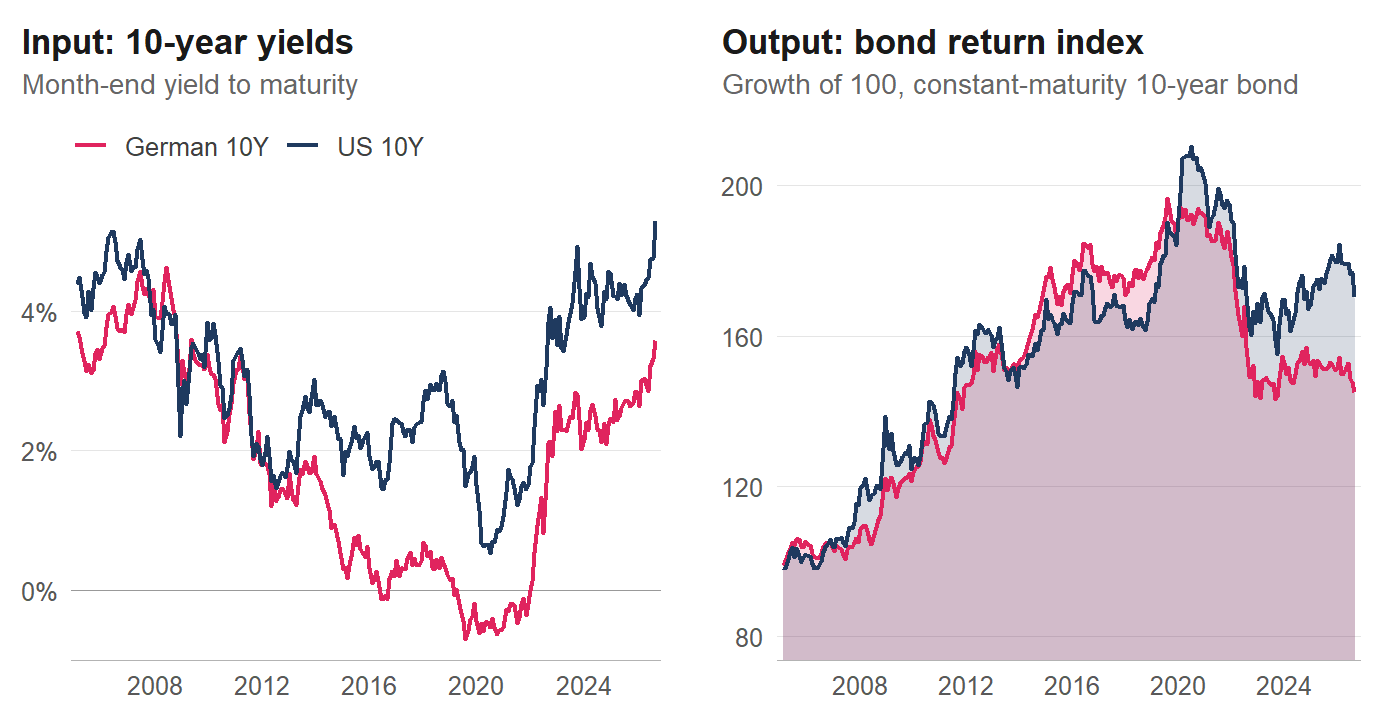
\includegraphics[width=1\linewidth]{Question4_files/figure-latex/bonds-1} 

}

\caption{Ten-year government bond yields (left) and the constructed return indexes (right) \label{bonds}}\label{fig:bonds}
\end{figure}

\section{Method}\label{method}

At each quarter-end from December 2019, the fund is re-optimised using
all monthly data since January 2010, an expanding window that always
spans at least ten years. Only assets with at least five years of
returns are eligible, so Large and Mid Caps (which start in 2015) become
eligible exactly at the first rebalance, Momentum from 2022 and Value
from 2023. Because these assets have shorter histories, correlations are
estimated pairwise and the covariance matrix is shrunk towards a
constant-correlation target (Ledoit and Wolf, 2004), which stabilises
the estimate. Historical average returns are notoriously noisy, so they
are shrunk halfway towards the cross-sectional average. All mandate
limits enter a quadratic programme as linear constraints, and three
strategies are compared:

\begin{itemize}
\tightlist
\item
  \textbf{Minimum variance}, which uses only the covariance matrix;
\item
  \textbf{Maximum Sharpe ratio}, found by tracing the constrained
  efficient frontier and choosing the portfolio with the highest
  expected excess return per unit of risk;
\item
  \textbf{Naive (equal weight)}, the feasible portfolio closest to equal
  weights, as a benchmark that requires no estimates at all.
\end{itemize}

Weights apply from the month after each rebalance and drift with returns
until the next one.

\section{What does the mandate cost?}\label{what-does-the-mandate-cost}

Figure \ref{frontier} compares the efficient frontier at the latest
rebalance with and without the mandate's limits (keeping only the
long-only rule). The shaded gap is the cost of the mandate: about
0.3-0.5 percentage points of expected return at the same level of risk,
and a fall in the best achievable Sharpe ratio from 0.43 to 0.38. More
strikingly, the mandate removes the entire low-risk end of the frontier.
Without it, the least risky portfolio has a volatility of under 5\%;
with it, nothing below about 9\% is possible, because capping bonds at
25\% and commodities at 15\% forces at least 60\% into equities. The
unconstrained maximum-Sharpe portfolio would hold about 71\% in local
bonds, so the bond cap is the expensive rule.

\begin{figure}[H]

{\centering 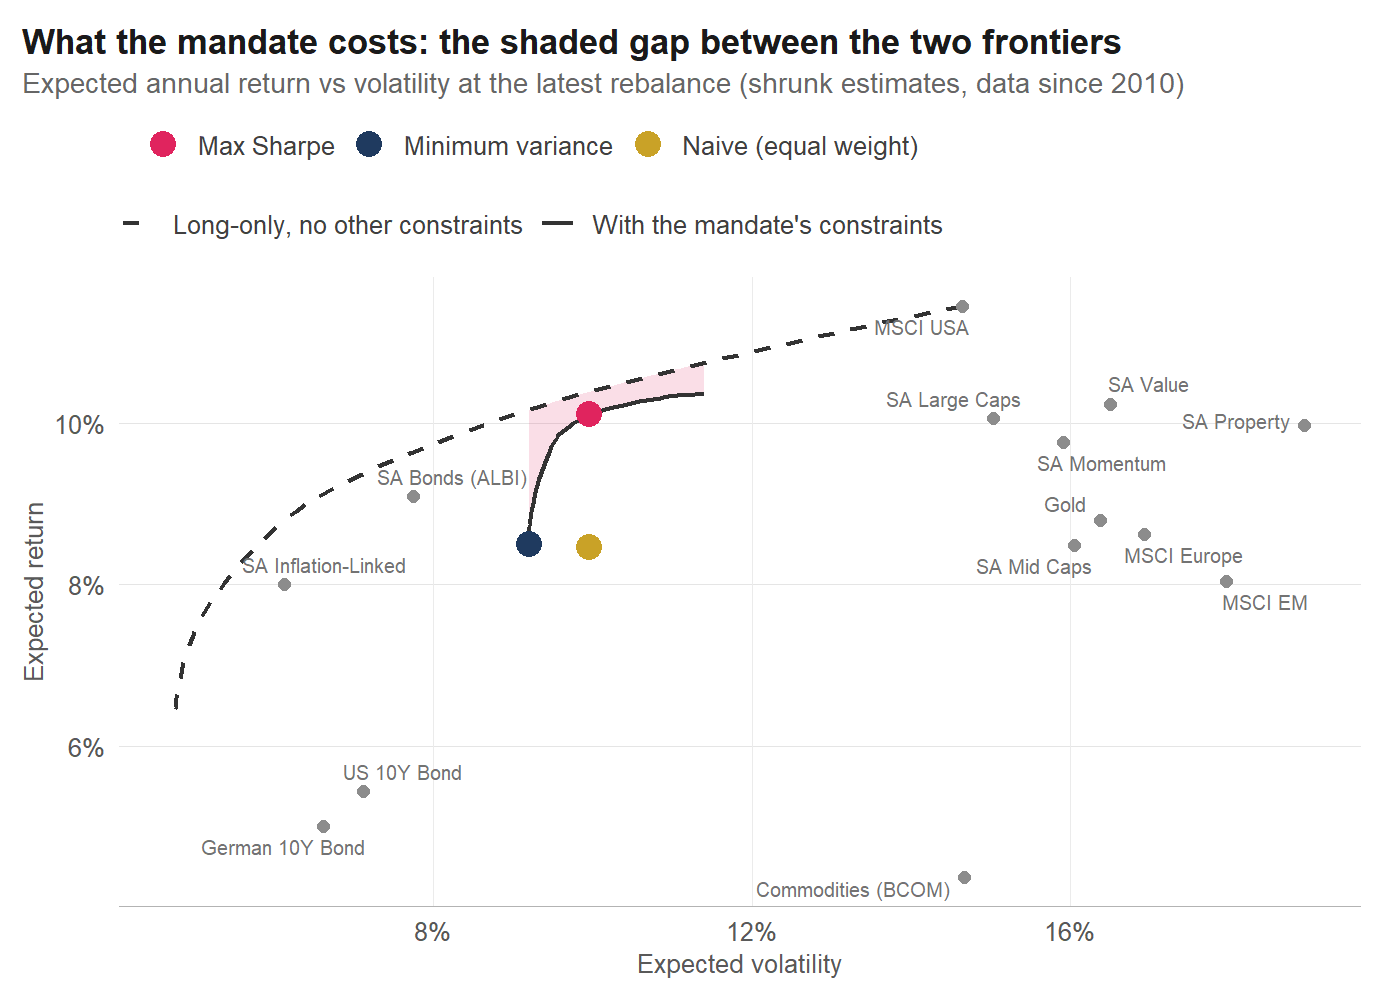
\includegraphics[width=1\linewidth]{Question4_files/figure-latex/frontier-1} 

}

\caption{Efficient frontiers with and without the mandate's constraints \label{frontier}}\label{fig:frontier}
\end{figure}

\section{Which rules shape the
portfolio?}\label{which-rules-shape-the-portfolio}

The quadratic programme returns a Lagrange multiplier for every
constraint: a positive multiplier (a ``shadow price'') means the
constraint is binding, so relaxing it would improve the objective.
Figure \ref{binding} shows which mandate rules bind at each rebalance.
The bond cap binds at every rebalance for all three strategies,
confirming that the mandate keeps the fund more equity-heavy than an
optimiser would choose. The minimum-variance fund also presses against
the commodity cap and the 60\% global limit throughout, as
low-correlation global bonds and commodities are its preferred
diversifiers. The maximum-Sharpe fund is pinned at the 35\% cap on MSCI
USA, the asset with the highest estimated return, which shows that the
single-asset cap is what stops it from concentrating in US equities.

\begin{figure}[H]

{\centering 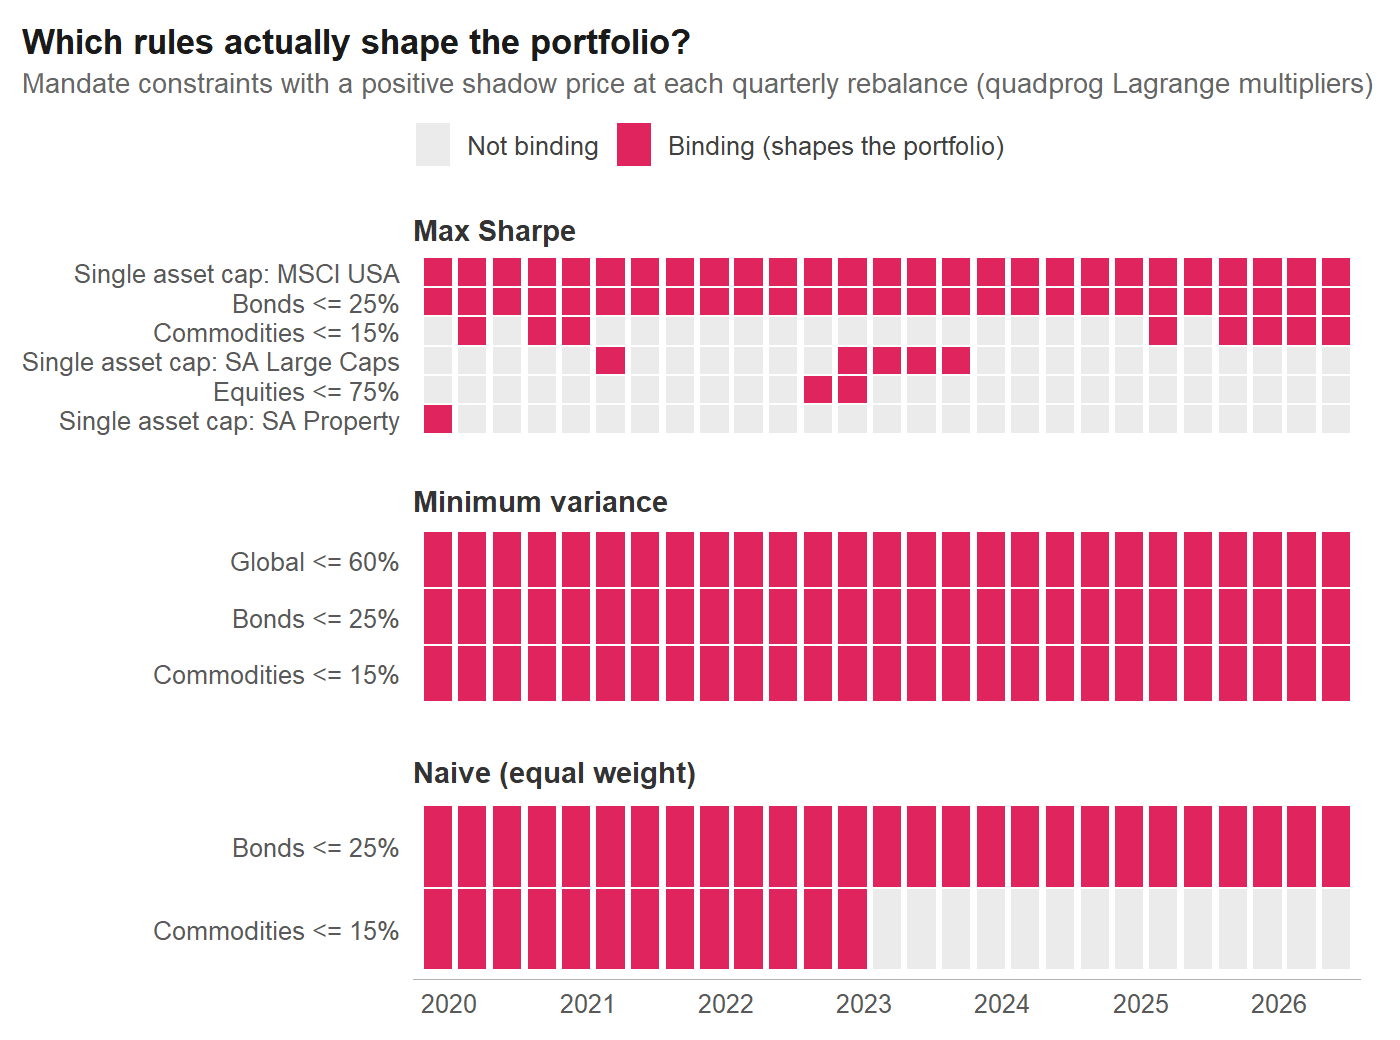
\includegraphics[width=1\linewidth]{Question4_files/figure-latex/binding-1} 

}

\caption{Binding mandate constraints at each quarterly rebalance \label{binding}}\label{fig:binding}
\end{figure}

\section{The portfolios}\label{the-portfolios}

Figure \ref{weights} shows how each strategy allocates across asset
groups over time, and Figure \ref{donuts} the latest allocation. The
maximum-Sharpe fund holds 25\% local bonds and no global bonds,
concentrating its equity in MSCI USA and local large caps. The
minimum-variance fund is the most diversified across asset classes, with
20\% in global bonds and 15\% in commodities alongside its equity. The
naive fund stays close to equal weights, adjusted only where the bond
and commodity caps require it.

\begin{figure}[H]

{\centering 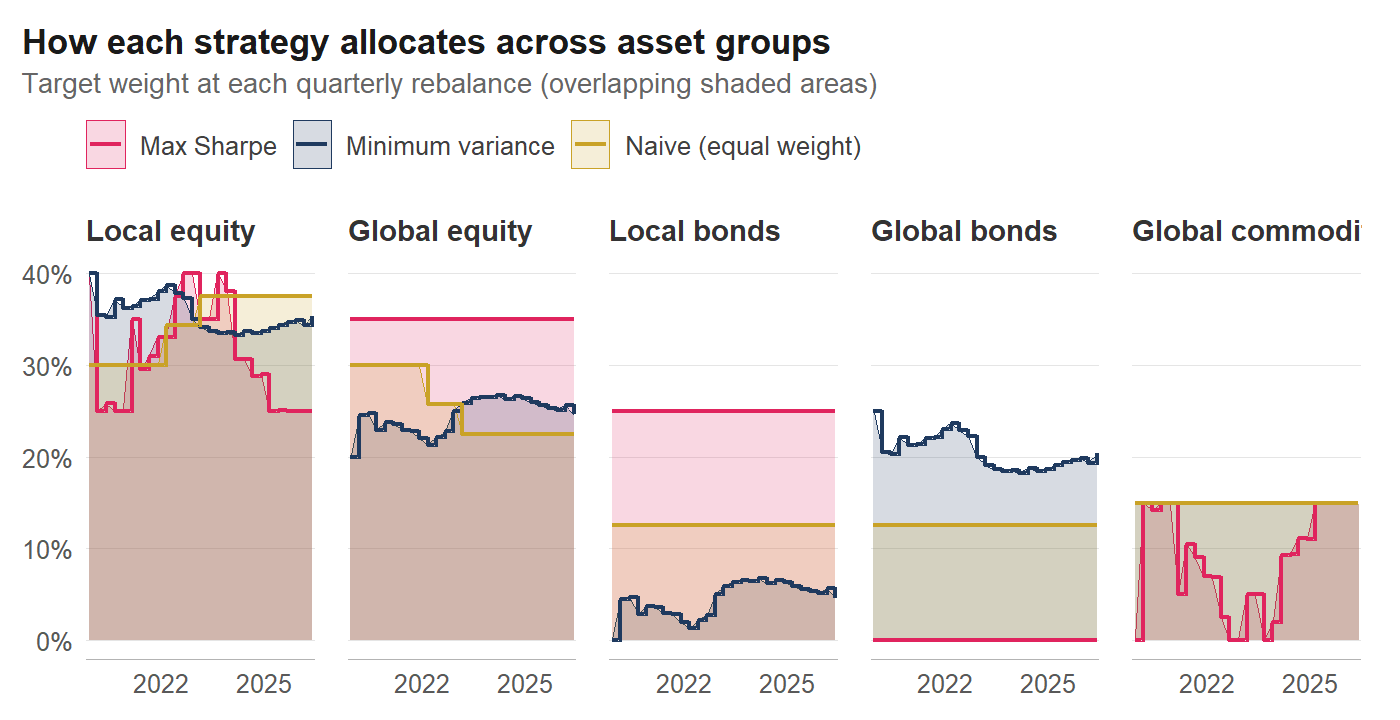
\includegraphics[width=1\linewidth]{Question4_files/figure-latex/weights-1} 

}

\caption{Asset-group weights at each rebalance \label{weights}}\label{fig:weights}
\end{figure}

\begin{figure}[H]

{\centering 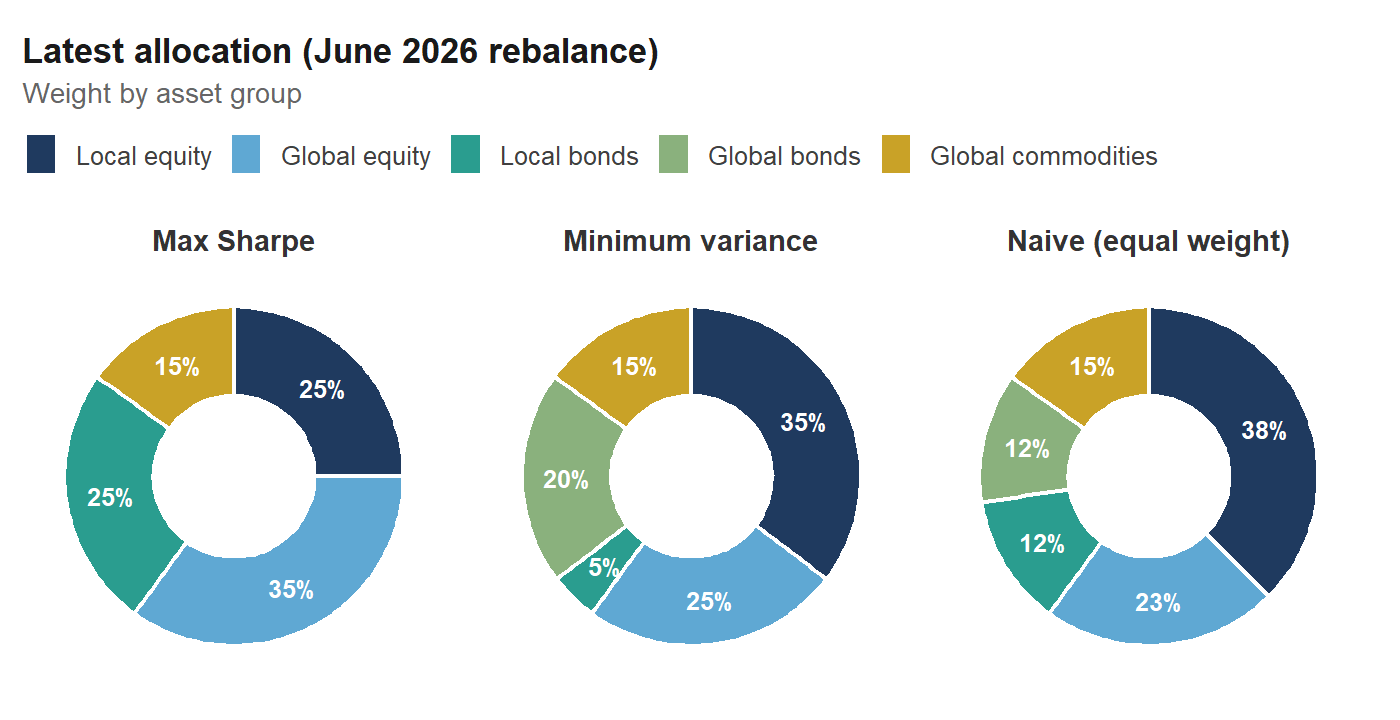
\includegraphics[width=1\linewidth]{Question4_files/figure-latex/donuts-1} 

}

\caption{Latest allocation by asset group \label{donuts}}\label{fig:donuts}
\end{figure}

\section{Out-of-sample performance}\label{out-of-sample-performance}

Table \ref{tab:stats} and Figure \ref{perf} summarise performance from
January 2020 to September 2026. The maximum-Sharpe fund earned the
highest return (11.8\% a year), but with the highest volatility and by
far the deepest drawdown (-23\% in the COVID-19 crash). The
minimum-variance fund earned almost as much (11.1\%) with much less
risk, giving the best Sharpe ratio and a maximum drawdown of only -14\%.
Both optimised funds beat the naive benchmark, which earned 9.8\% a
year. The cost of optimisation is turnover: the optimised funds trade
about 5\% of the portfolio per quarter on average against under 1\% for
the naive fund, with large rebalances in 2020 as the COVID-19 shock
changed the estimated covariances.

\begin{table}[H]
\centering
\caption{Out-of-sample performance, January 2020 - September 2026 (returns, volatility, drawdown and quarterly turnover in \%) \label{tab:stats}} 
\begin{tabular}{lrrrrrr}
  \toprule
Strategy & Ann. return & Ann. volatility & Sharpe & Max drawdown & Worst month & Avg. turnover \\ 
  \midrule
Max Sharpe & 11.80 & 13.48 & 0.43 & -23.38 & -16.09 & 5.15 \\ 
  Minimum variance & 11.12 & 10.82 & 0.45 & -14.10 & -7.36 & 4.88 \\ 
  Naive (equal weight) & 9.81 & 11.68 & 0.33 & -18.29 & -13.17 & 0.62 \\ 
   \bottomrule
\end{tabular}
\end{table}

\begin{figure}[H]

{\centering 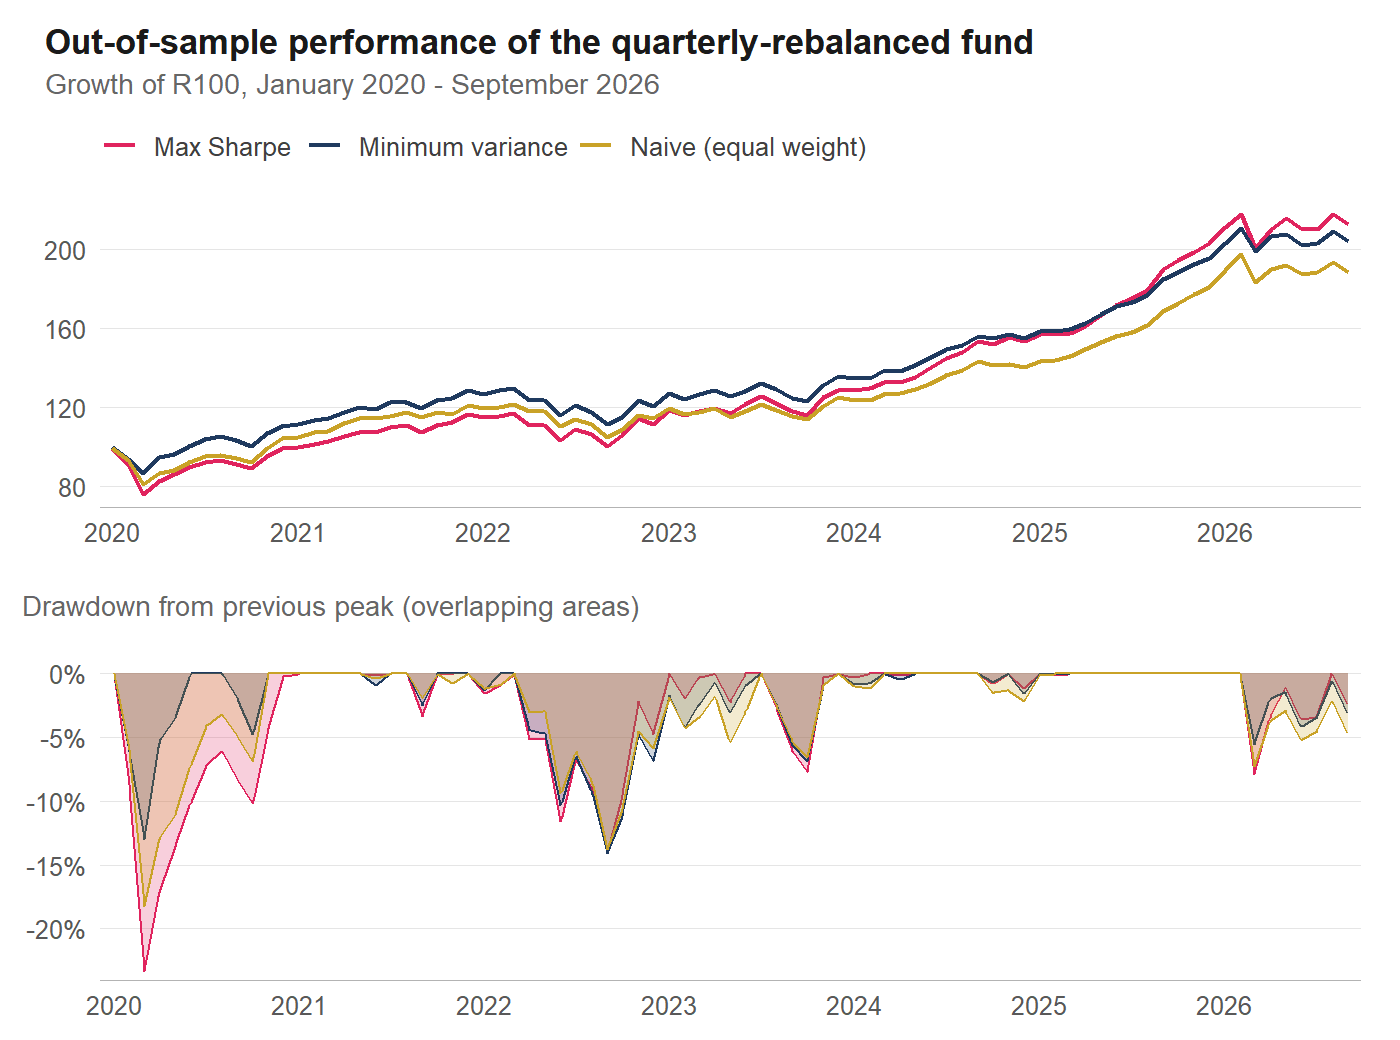
\includegraphics[width=1\linewidth]{Question4_files/figure-latex/perf-1} 

}

\caption{Growth of R100 and drawdowns \label{perf}}\label{fig:perf}
\end{figure}

Figure \ref{violins} looks at the shape of the monthly returns. The
three funds have similar typical months, but their left tails differ:
the minimum-variance fund's returns are close to symmetric (skewness of
-0.36), while the maximum-Sharpe and naive funds show long left tails
(skewness of -1.27 and -1.09) driven by sharp losses in equity
sell-offs.

\begin{figure}[H]

{\centering 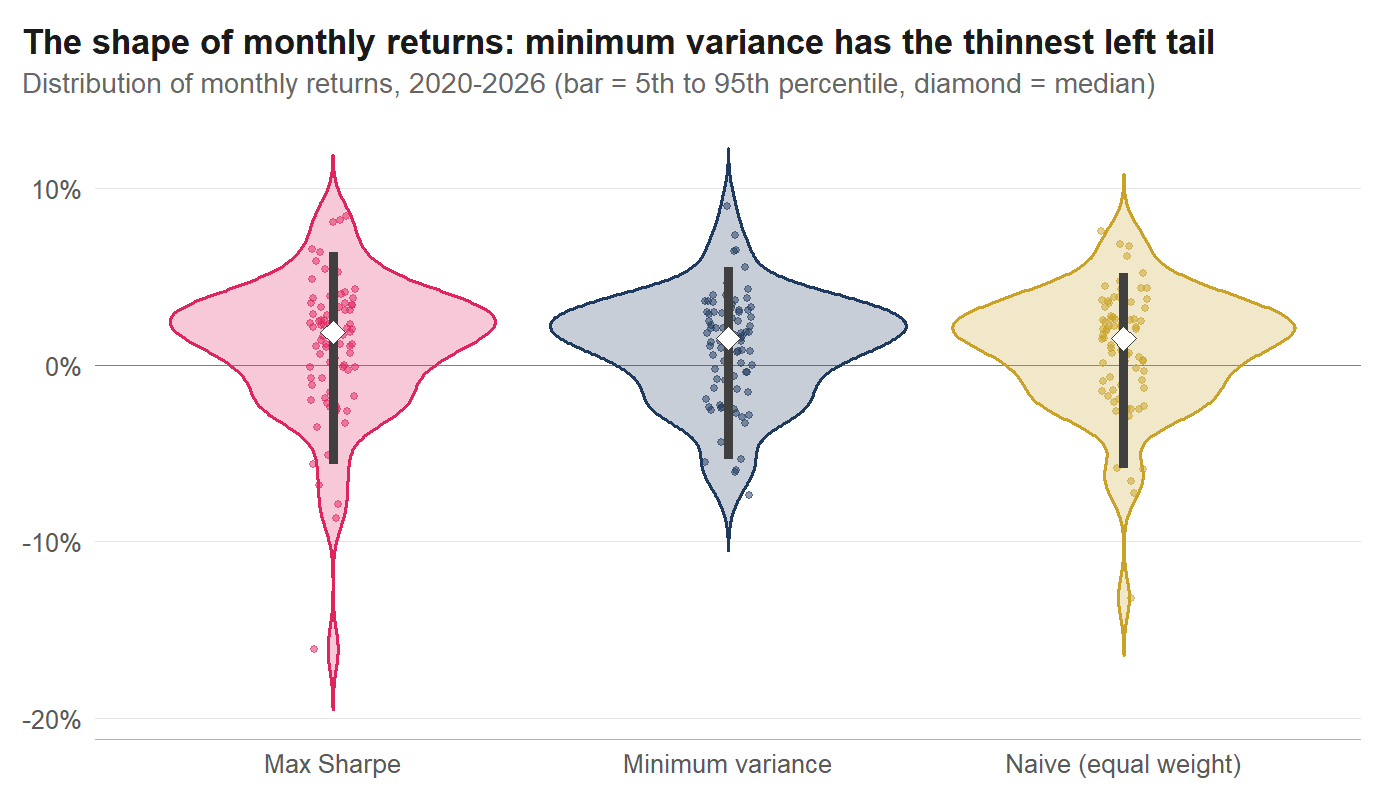
\includegraphics[width=1\linewidth]{Question4_files/figure-latex/violins-1} 

}

\caption{Distribution of monthly returns \label{violins}}\label{fig:violins}
\end{figure}

\section{\texorpdfstring{Conclusion
\label{Conclusion}}{Conclusion }}\label{conclusion}

A global balanced index fund can be built from the available indexes
within the mandate, and quarterly optimisation adds value over simple
equal weighting. The minimum-variance fund is the most attractive: it
delivered nearly the highest return with the lowest volatility, the
smallest drawdown and the most symmetric return profile, and it relies
only on covariance estimates, which are far more reliable than return
forecasts. The mandate itself, however, deserves scrutiny. Its 25\% bond
cap binds at every rebalance, rules out the low-risk part of the
efficient frontier and costs about 0.3-0.5 percentage points of expected
return at a given level of risk; for a fund described as balanced, a
higher bond limit would be worth considering. Two caveats apply: global
assets are measured in US dollars because no exchange rate is available,
so the rand's effect on returns is not captured, and the out-of-sample
period of under seven years includes only one major sell-off.

\bibliography{Tex/ref}





\end{document}
